\documentclass[11pt,a4paper]{article}
\usepackage[margin=0.75in]{geometry}
\usepackage[english]{babel}
\usepackage[utf8x]{inputenc}
\usepackage{amsmath}
\usepackage{graphicx}
\usepackage{upgreek}
\usepackage{caption}
\usepackage{relsize}
\usepackage{booktabs}
\usepackage{float}
\usepackage{multicol}
\usepackage{tikz}
\usepackage{fancyhdr}
\usepackage{listings}
\usepackage{courier}
\usepackage[hidelinks]{hyperref}
\usepackage{titlesec}
\usepackage{subfiles}
\usepackage[subpreambles=true]{standalone}
\usepackage{import}
\setlength{\parindent}{0in}
\setlength{\parskip}{1em}
\titlespacing*{\section}{0pt}{1ex}{1ex}
\titlespacing*{\subsection}{0pt}{0.5ex}{0.5ex}
\titlespacing*{\subsubsection}{0pt}{0.5ex}{0.5ex}
\usepackage{csquotes}
\renewcommand{\lstlistingname}{Code}
\hypersetup{
	bookmarks=true,         
	unicode=true,         
	pdftoolbar=false,        
	pdfmenubar=false,        
	pdffitwindow=false,     
	pdfstartview={FitH},    
	pdftitle={Assignment 2 - Manan, Anirudh BH}, 
	pdfauthor={Manan Sharma, Anirudh BH},
	pdfnewwindow=true,      
}
\graphicspath{ {./images/} }
\lstset{basicstyle = \small\ttfamily, language=Verilog, frame=single, breaklines=true}
\begin{document}
	\cleardoublepage
	
	\subfile{frontpage}
	\thispagestyle{empty}
	
	\section*{Question 1}
	Construct an FSM that checks if a binary number is divisible by 3. Specifically, your FSM should take input bits sequentially starting from LSB and output REM= 1 if the number is not divisible and REM = 0 if the number is divisible. Write a synthesisable Verilog code for the same.
	\begin{figure}[H]
		\centering
		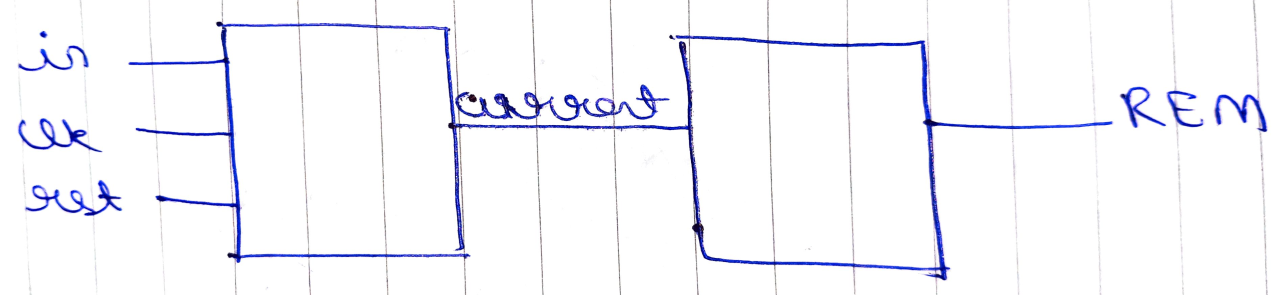
\includegraphics[width=1\linewidth]{images/q1blockdiag}
		\caption[]{Block Diagram for Q1}
		\label{fig:q1blck}
	\end{figure}
	\begin{figure}[H]
		\centering
		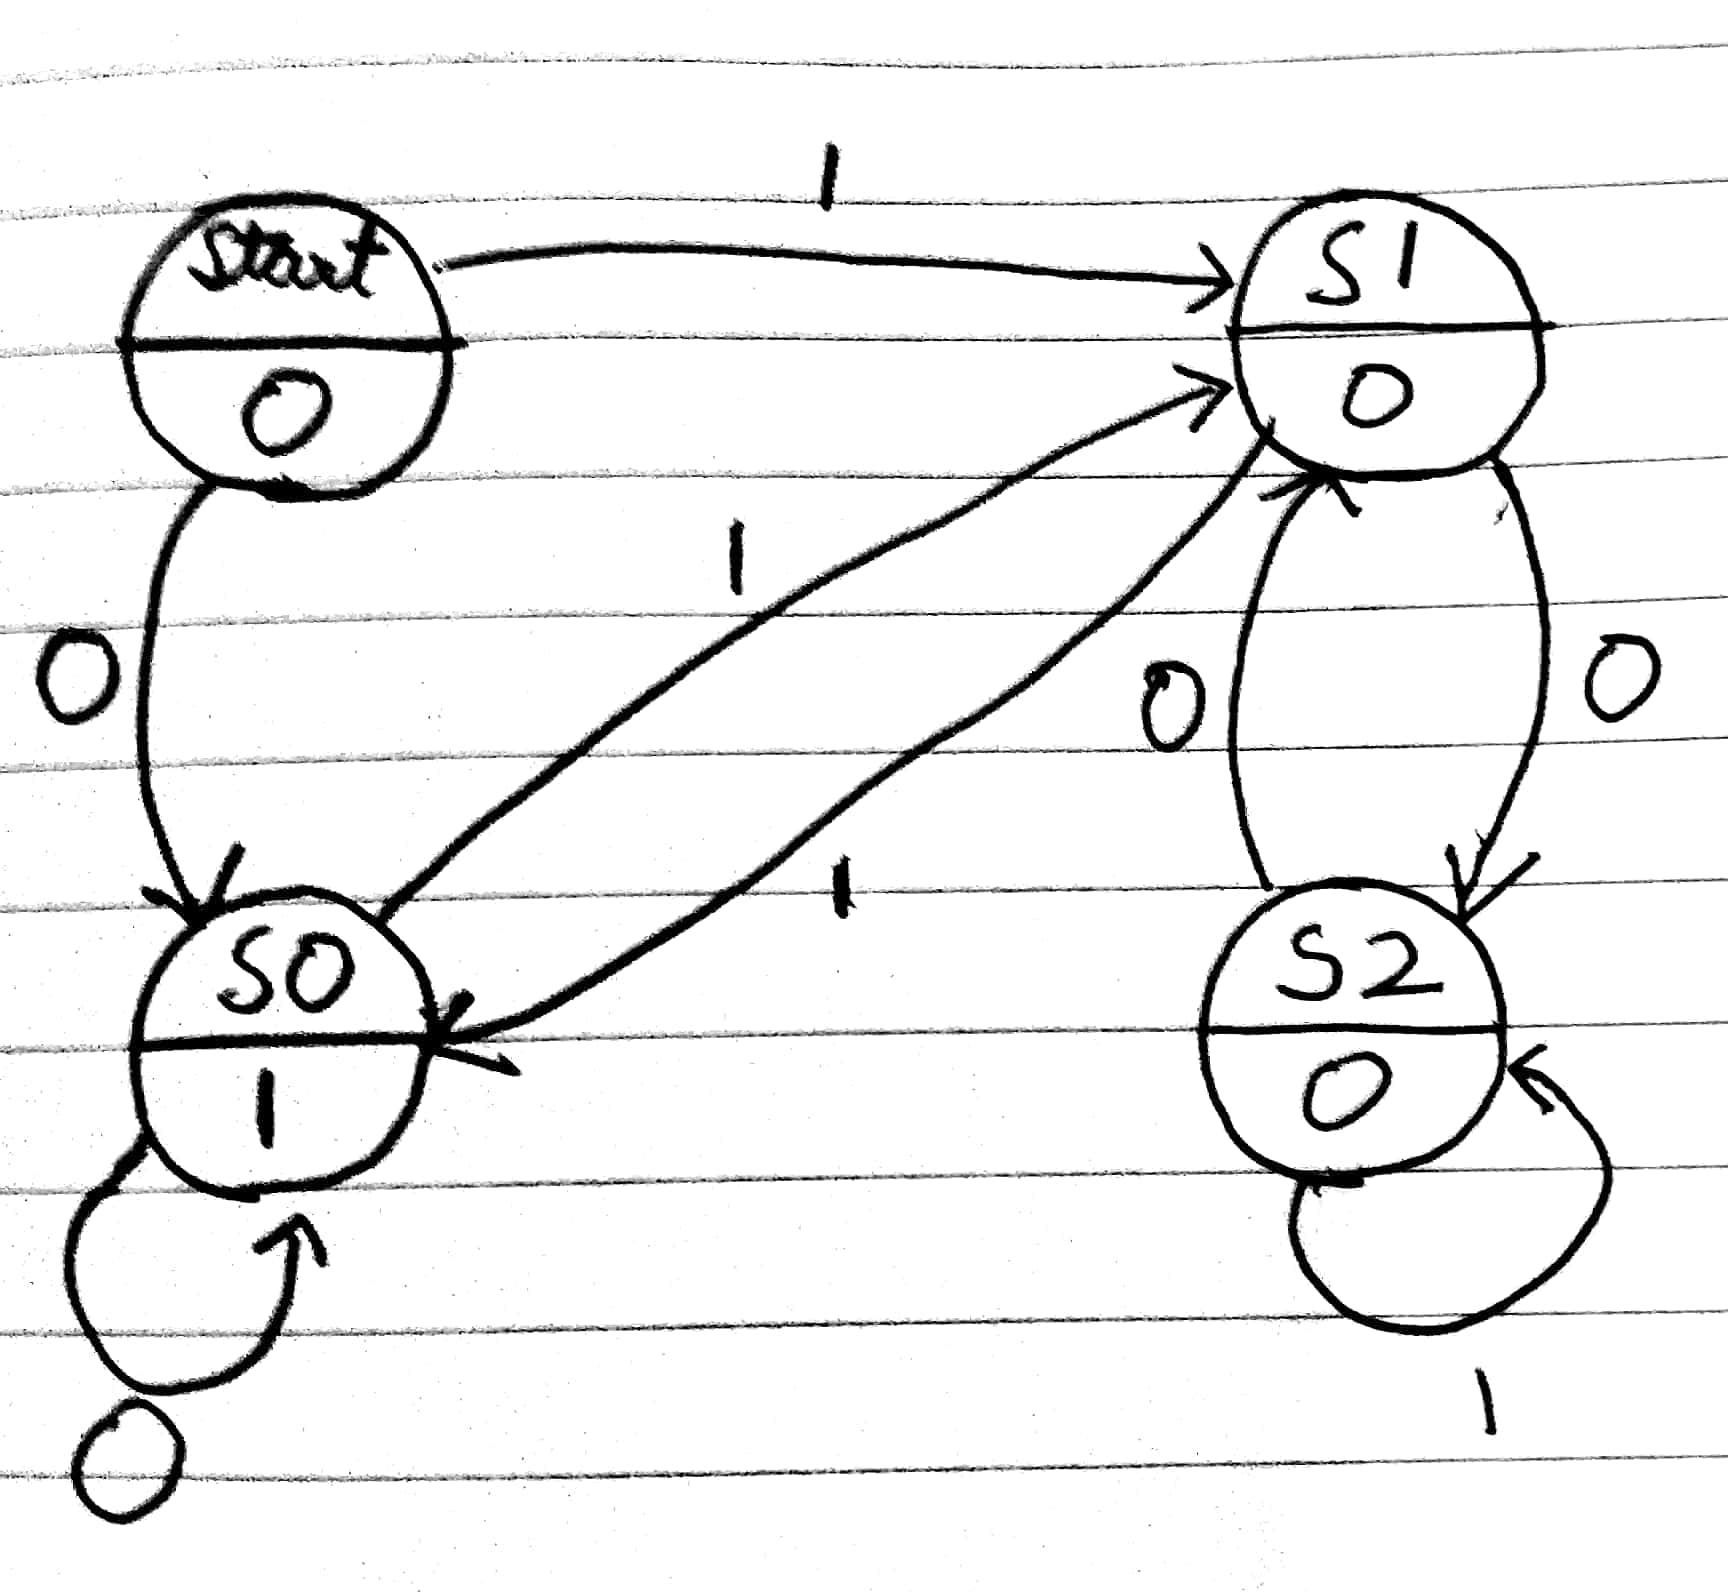
\includegraphics[scale=0.1]{images/q1fsm}
		\caption[]{FSM for Q1}
		\label{fig:q1fsm}
	\end{figure}
	\lstinputlisting[caption={Verilog Code for Q1}]{codes/q1.v}
	
	\begin{figure}[H]
		\centering
		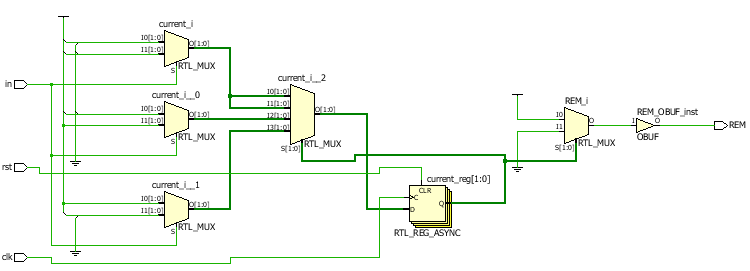
\includegraphics[width=1\linewidth]{images/q1elaborated}
		\caption[]{Elaborated Design for Q1}
		\label{fig:q1elaborated}
	\end{figure}
	
	\lstinputlisting[caption={Testbench for Question 1}]{codes/q1testbench.v}
	\begin{figure}[H]
		\centering
		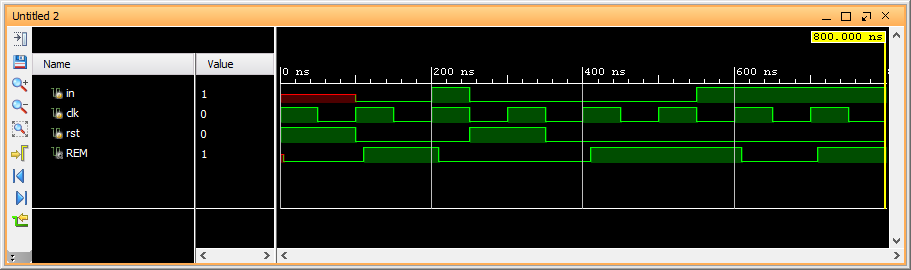
\includegraphics[width=1\linewidth]{images/q1output}
		\caption[]{Post Implementation Output for Q1}
		\label{fig:q1output}
	\end{figure}
	\begin{figure}[H]
		\centering
		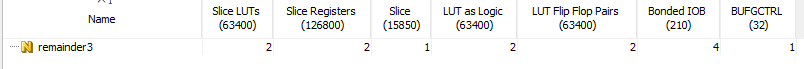
\includegraphics[width=1\linewidth]{images/q1utilization}
		\caption[]{Resource Utilization for Q1}
		\label{fig:q1utilization}
	\end{figure}
	 
	 
	 \section*{Question 2}
	 Design a finite state machine for 8-bit restoring division. Write a synthesisable verilog code for the same.
	 \begin{figure}[H]
	 	\centering
	 	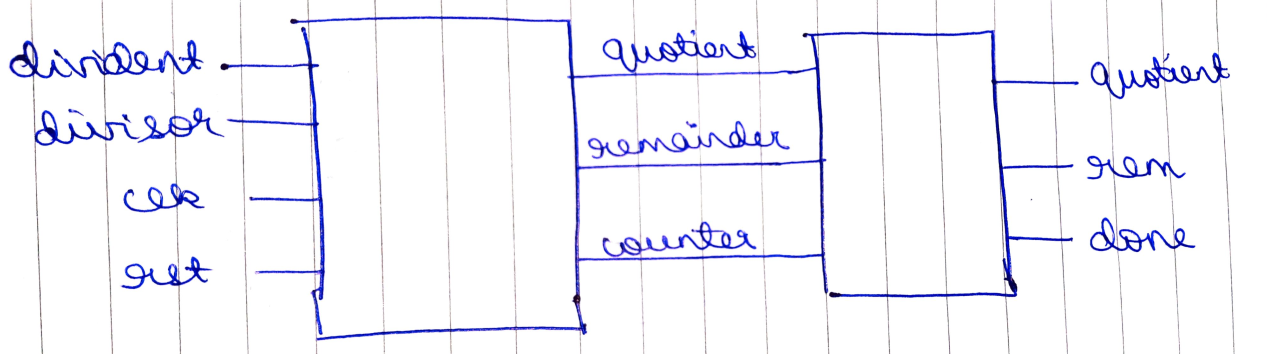
\includegraphics[width=1\linewidth]{images/q2blockdiag}
	 	\caption[]{Block Diagram for Q2}
	 	\label{fig:q2blck}
	 \end{figure} 
	 	\begin{figure}[H]
	 	\centering
	 	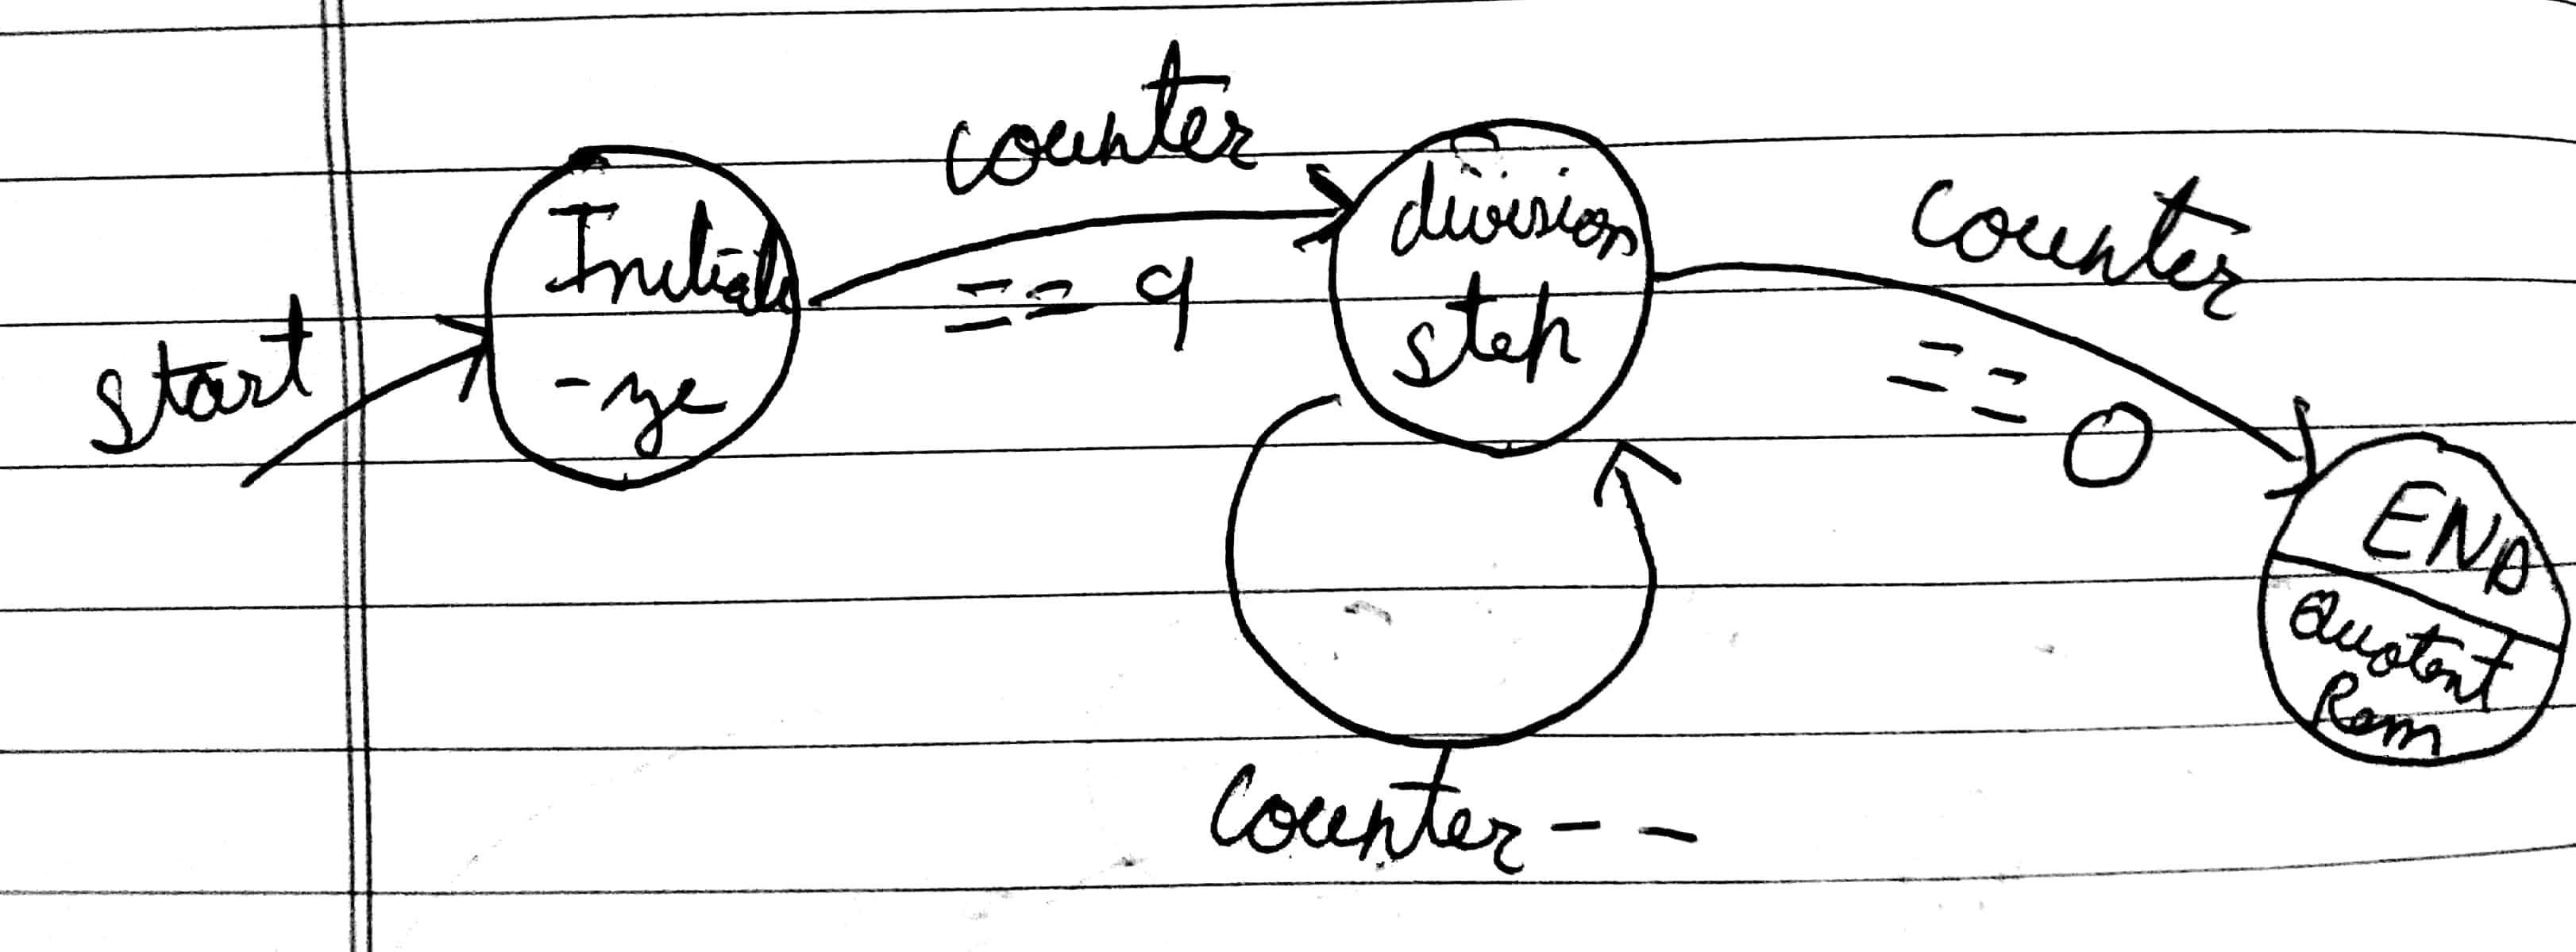
\includegraphics[scale=0.1]{images/q2fsm}
	 	\caption[]{FSM for Q2}
	 	\label{fig:q2fsm}
	 \end{figure}
	 \lstinputlisting[caption={Verilog Code for Q2}]{codes/q2.v}
	 \begin{figure}[H]
	 	\centering
	 	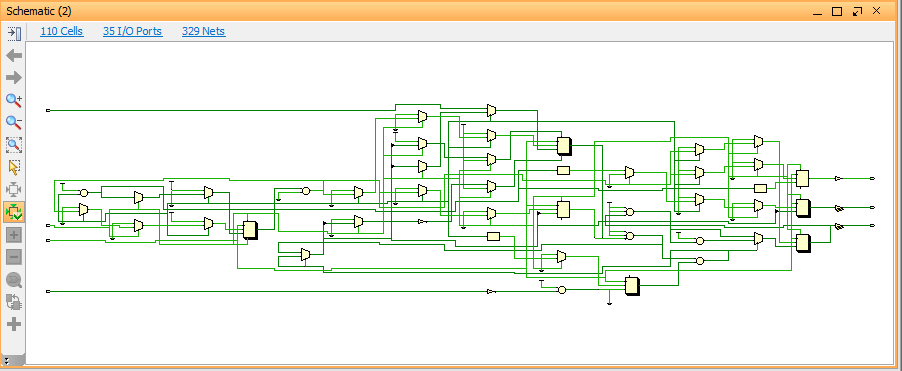
\includegraphics[width=1\linewidth]{images/q2elaborated}
	 	\caption[]{Elaborated Design for Q2}
	 	\label{fig:q2elaborated}
	 \end{figure}
	 \lstinputlisting[caption={Testbench for Q2}]{codes/q2testbench.v}
	 \begin{figure}[H]
	 	\centering
	 	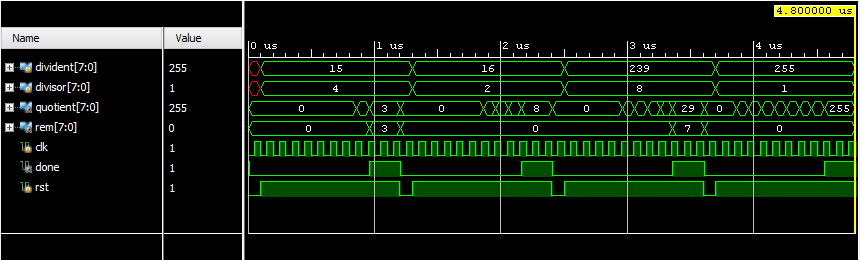
\includegraphics[width=1\linewidth]{images/q2output}
	 	\caption[]{Post Implementation Output for Q2}
	 	\label{fig:q2output}
	 \end{figure}
	 \begin{figure}[H]
	 	\centering
	 	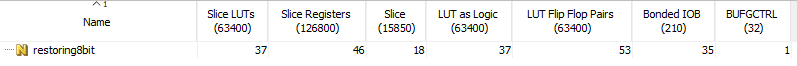
\includegraphics[width=1\linewidth]{images/q2utilization}
	 	\caption[]{Resource Utilization for Q2}
	 	\label{fig:q2utilization}
	 \end{figure}
	 
	  \section*{Question 3}
	 Design a finite state machine for 8-bit non restoring division. Write a synthesisable verilog code for the same. 
	 \begin{figure}[H]
	 	\centering
	 	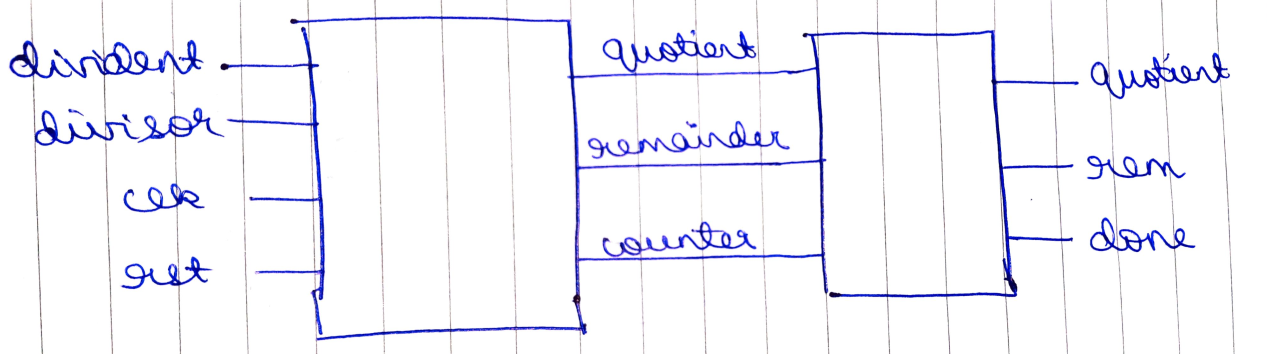
\includegraphics[width=1\linewidth]{images/q2blockdiag}
	 	\caption[]{Block Diagram for Q3}
	 	\label{fig:q3blck}
	 \end{figure}
	 	\begin{figure}[H]
	 	\centering
	 	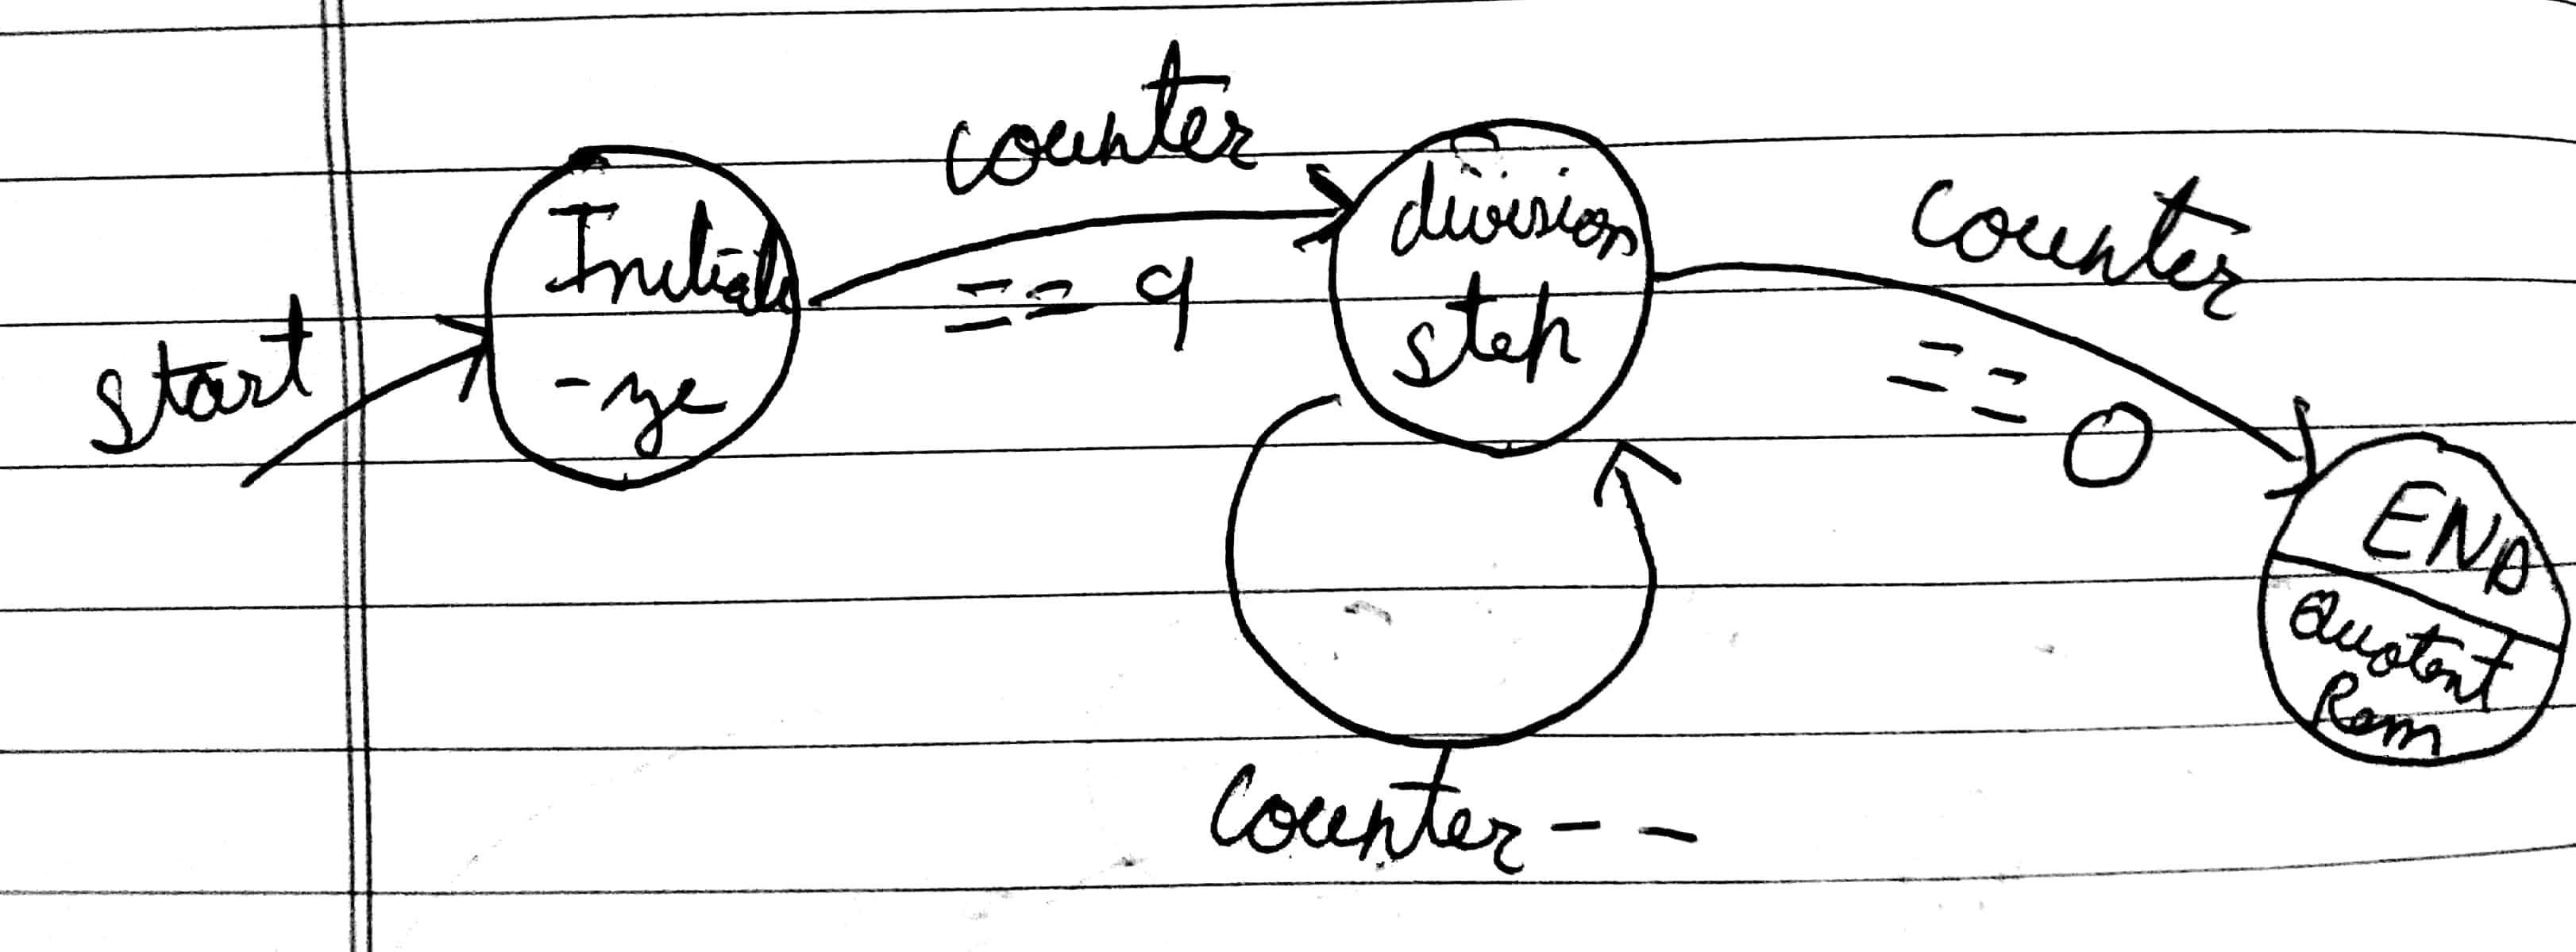
\includegraphics[scale=0.1]{images/q2fsm}
	 	\caption[]{FSM for Q3}
	 	\label{fig:q3fsm}
	 \end{figure}
	 \lstinputlisting[caption={Verilog Code for Q3}]{codes/q3.v}
	 \begin{figure}[H]
	 	\centering
	 	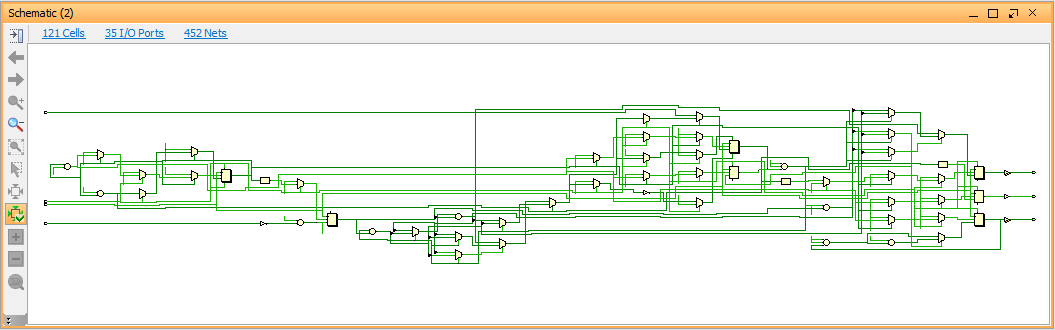
\includegraphics[width=1\linewidth]{images/q3elaborated}
	 	\caption[]{Elaborated Design for Q3}
	 	\label{fig:q3elaborated}
	 \end{figure}
	 \lstinputlisting[caption={Testbench for Q3}]{codes/q3testbench.v}
	 \begin{figure}[H]
	 	\centering
	 	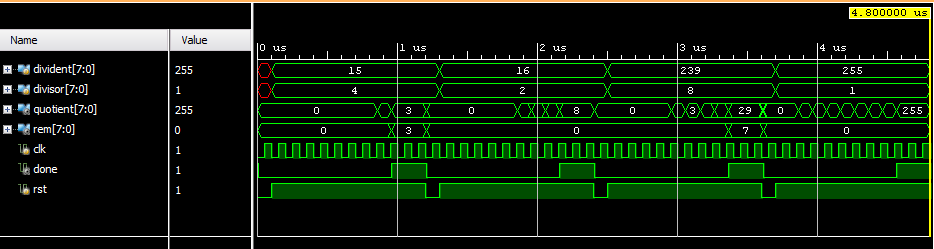
\includegraphics[width=1\linewidth]{images/q3output}
	 	\caption[]{Post Implementation Output for Q3}
	 	\label{fig:q3output}
	 \end{figure}
	 \begin{figure}[H]
	 	\centering
	 	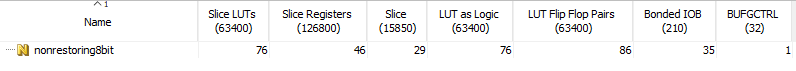
\includegraphics[width=1\linewidth]{images/q3utilization}
	 	\caption[]{Resource Utilization for Q3}
	 	\label{fig:q3utilization}
	 \end{figure}
 
 	\section*{Question 4}
 	Design a finite-state machine that illustrates the operation of a digital watch with two function buttons. Each successive push of button 1 causes the watch to change from displaying the time, to setting the hours, to setting the minutes and back to displaying the time again and so on. Button 2 allows the user to increment either the hours or the minutes when the watch is in the appropriate state.
	\begin{figure}[H]
		\centering
		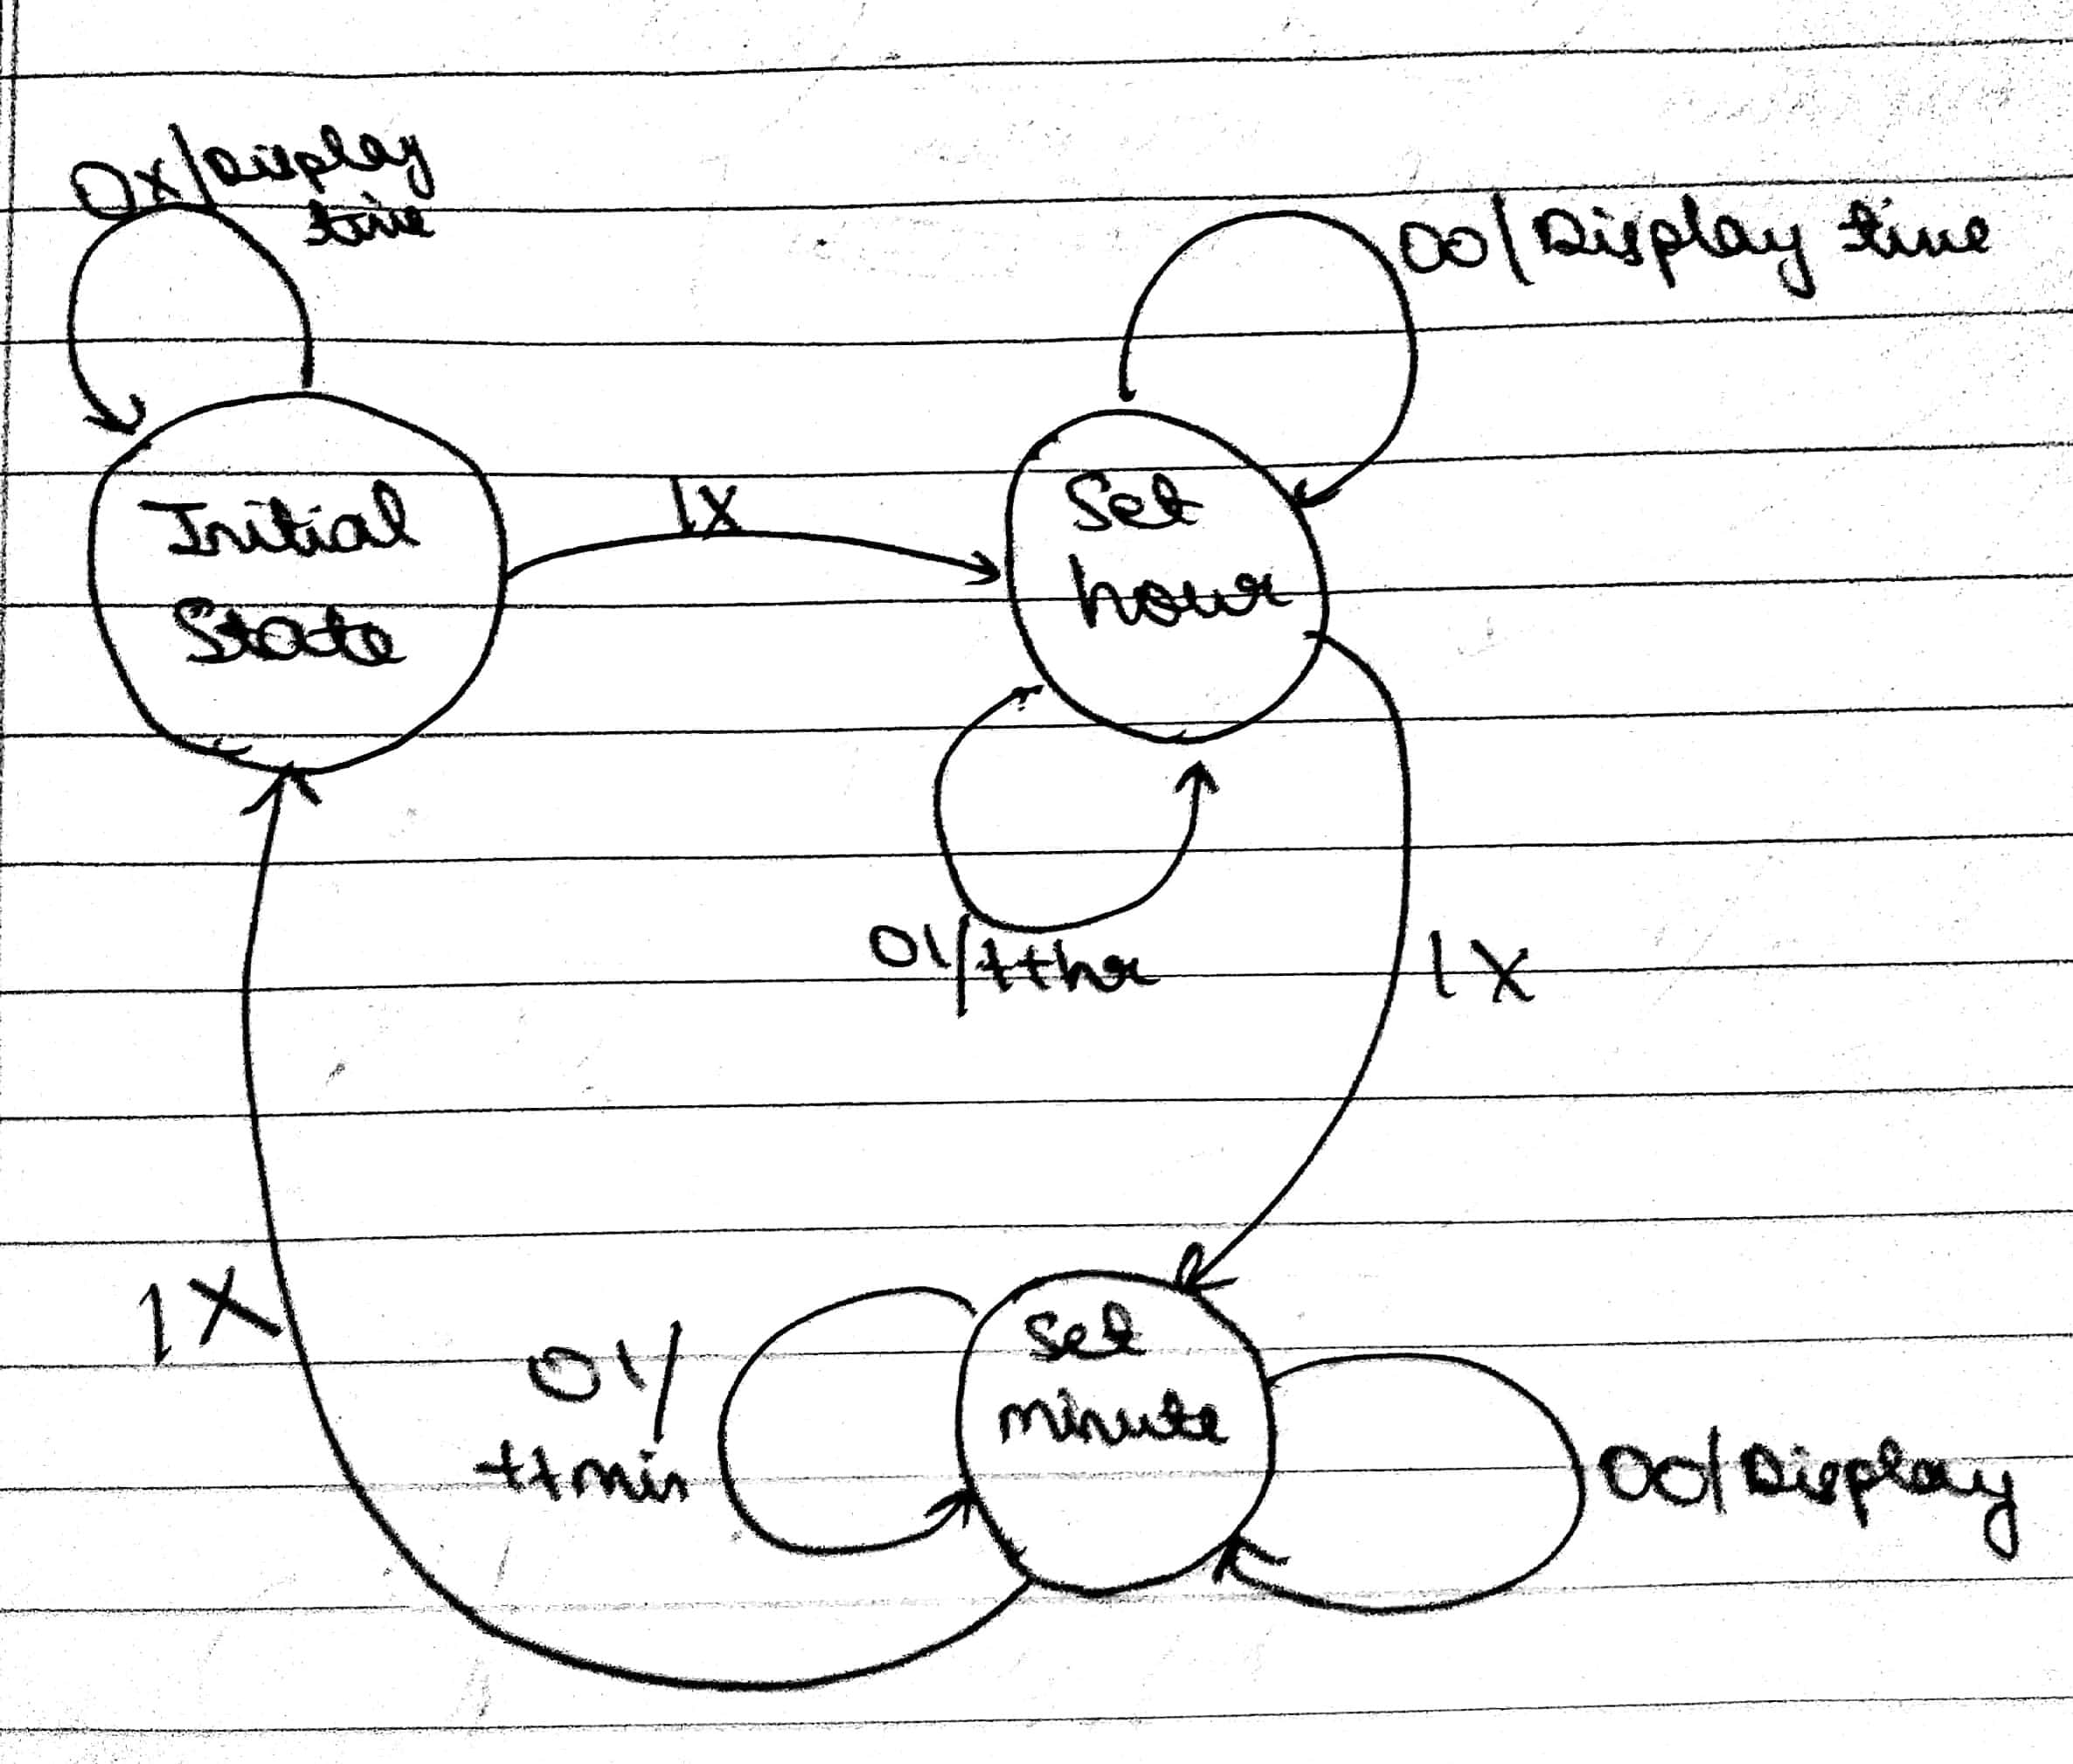
\includegraphics[scale=0.12]{images/q4fsm}
		\caption[]{FSM for Q4}
		\label{fig:q4fsm}
	\end{figure}
	
	\begin{figure}[H]
		\centering
		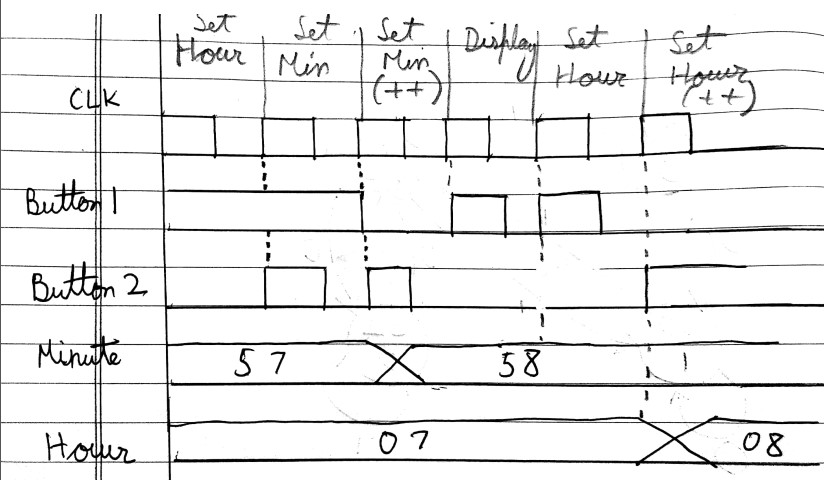
\includegraphics[width=1\linewidth]{images/q4timing}
		\caption[]{Timing Diagram for Q4}
		\label{fig:q4timing}
	\end{figure}
	\section*{Question 5}
	Design an FSM for a digital hardware circuit used to control an automatic teller machine that performs three tasks: tells the user the balance of his bank account, permits the user to withdraw an amount of money not greater than the balance on his account, and permits the user to deposit money into his account.
	
	\begin{figure}[H]
		\centering
		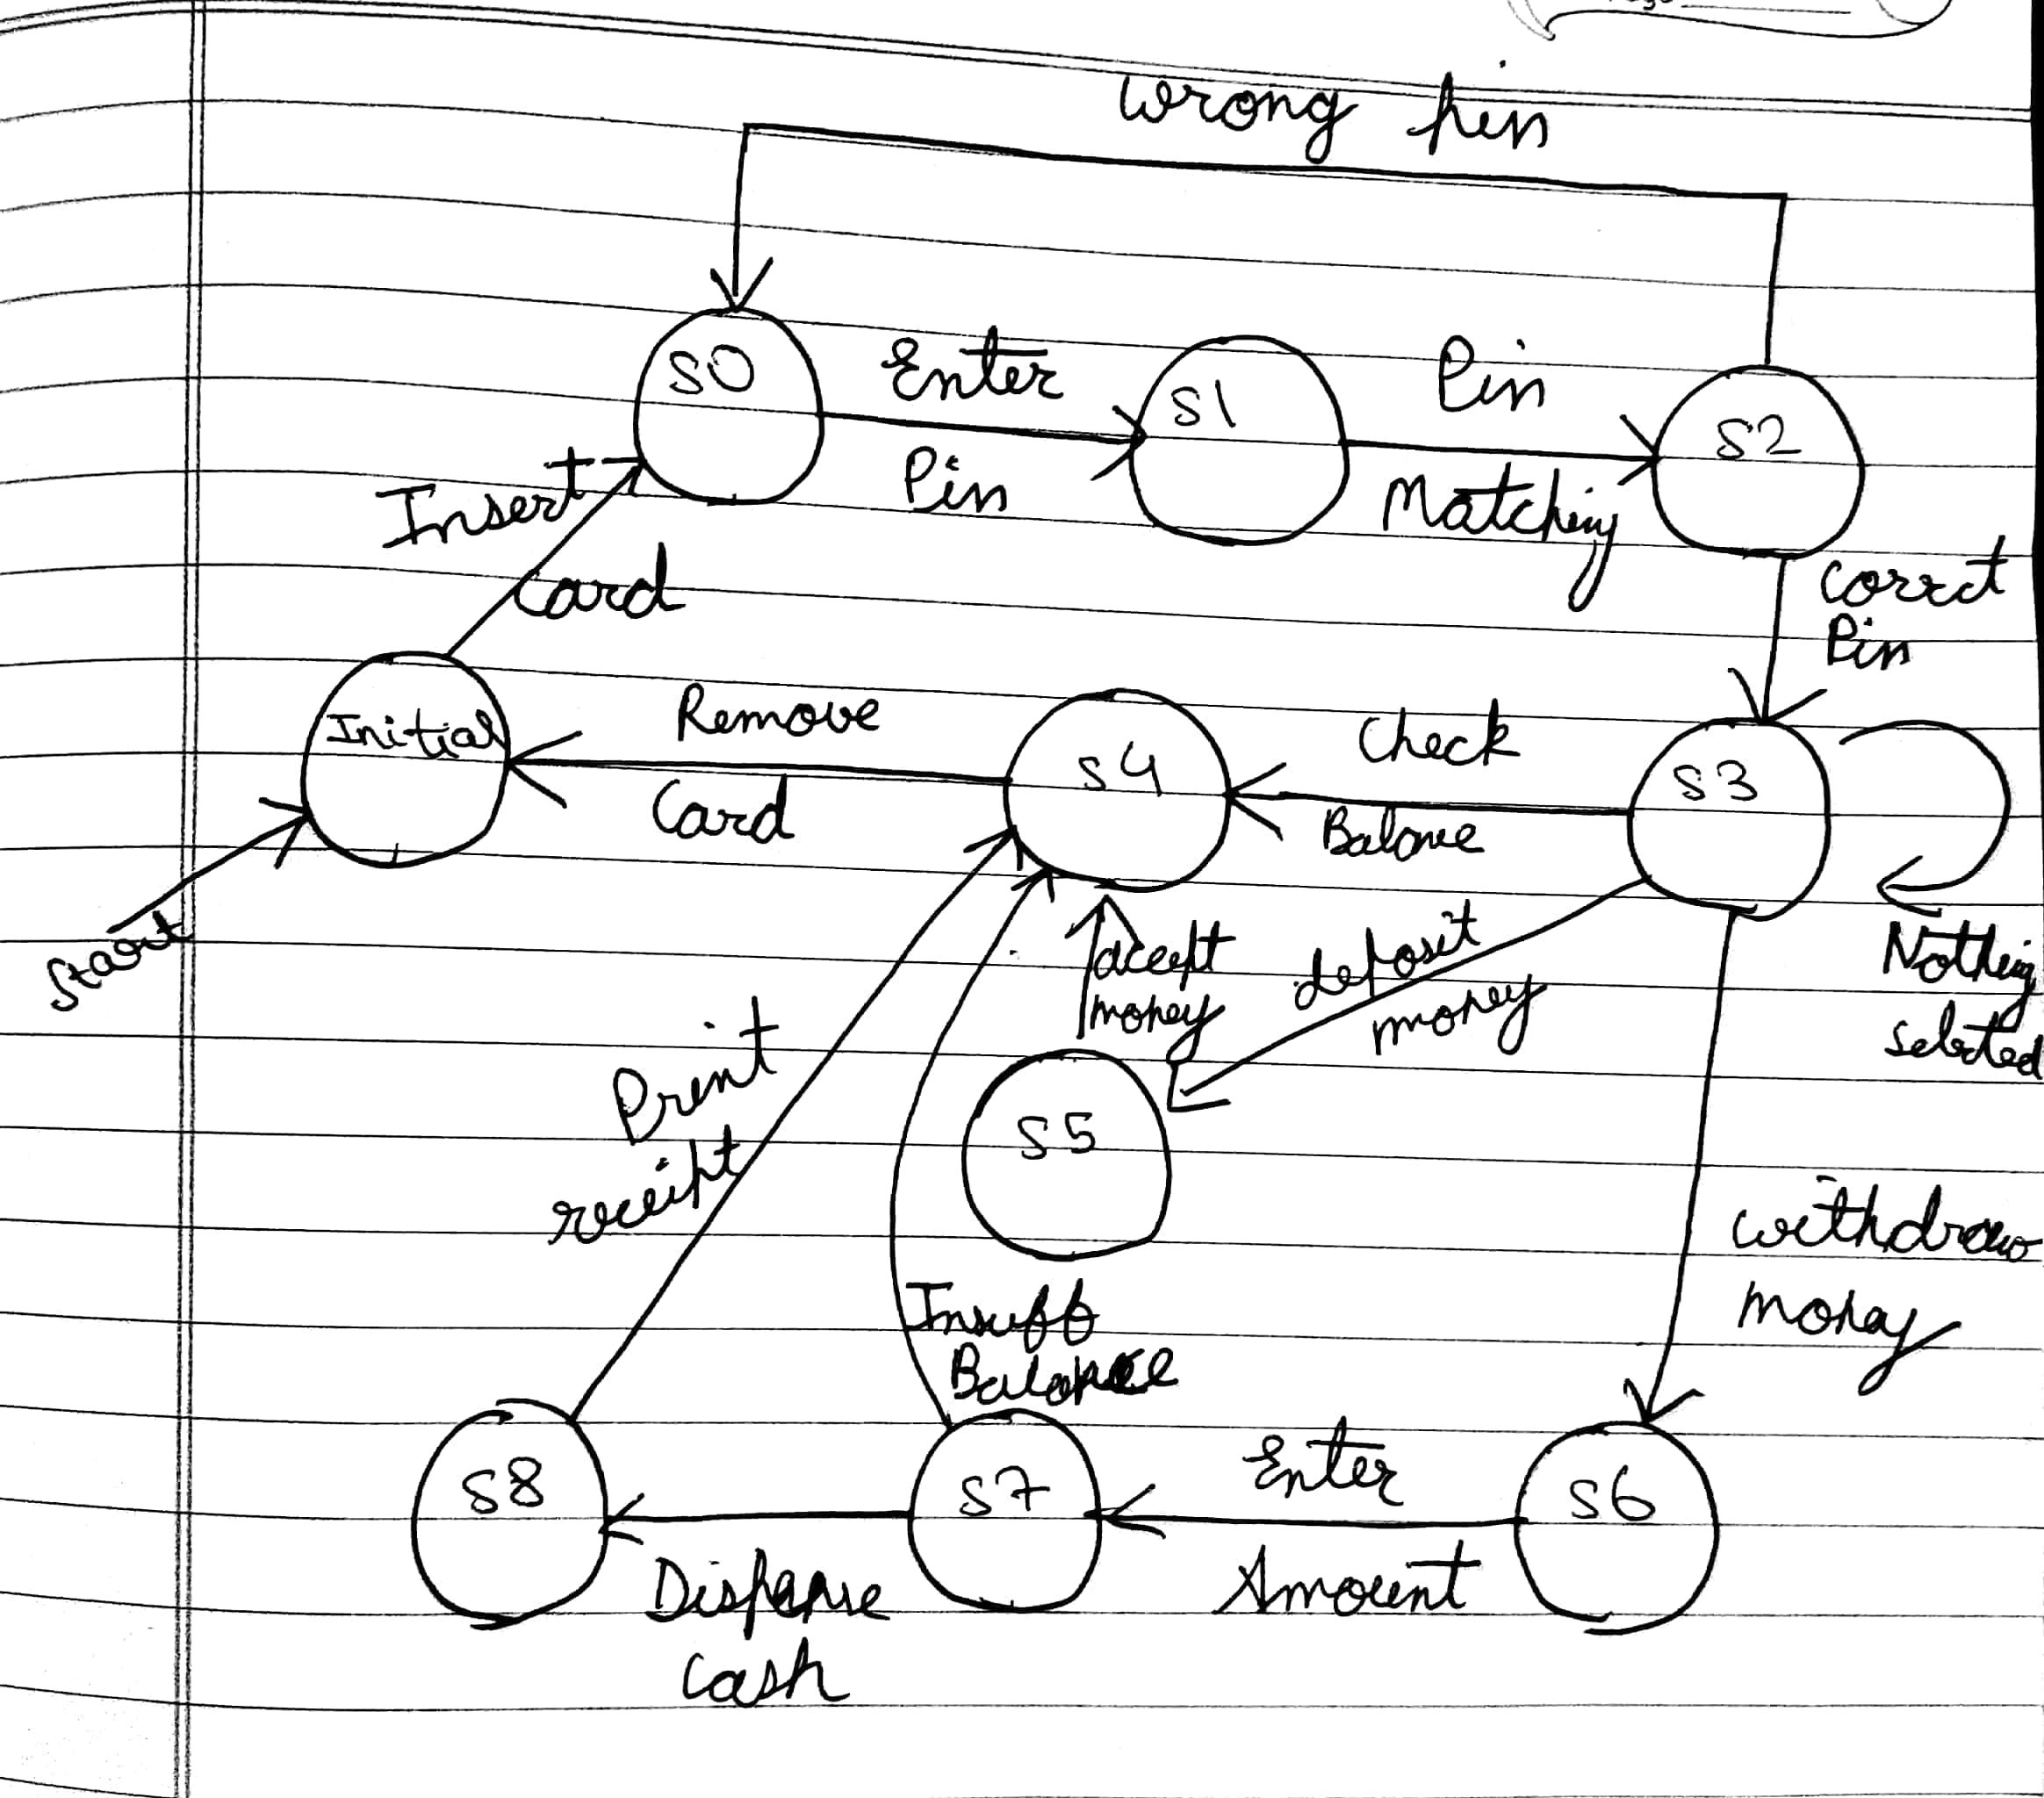
\includegraphics[scale=0.12]{images/q5fsm}
		\caption[]{FSM for Q5}
		\label{fig:q5fsm}
	\end{figure}

	\begin{figure}[H]
		\centering
		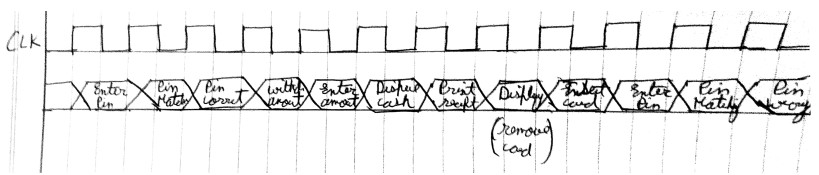
\includegraphics[width=1\linewidth]{images/q5timing}
		\caption[]{Timing Diagram for Q5}
		\label{fig:q5timing}
	\end{figure}
	\section*{Question 6}
	The overall objective is to create a line tracking robot. The system has two digital
	inputs and two digital outputs. You can simulate the system with two switches and two LEDs, or build a robot with two DC motors and two optical reflectance sensors. Both sensor inputs will be on if the machine is completely on the line. One sensor input will be on and the other off if the machine is just going off the track. If the machine is totally off the line, then both sensor inputs will be off. Implement the controller using a finite state machine. Choose a Moore or Mealy format as appropriate.
	\begin{figure}[H]
		\centering
		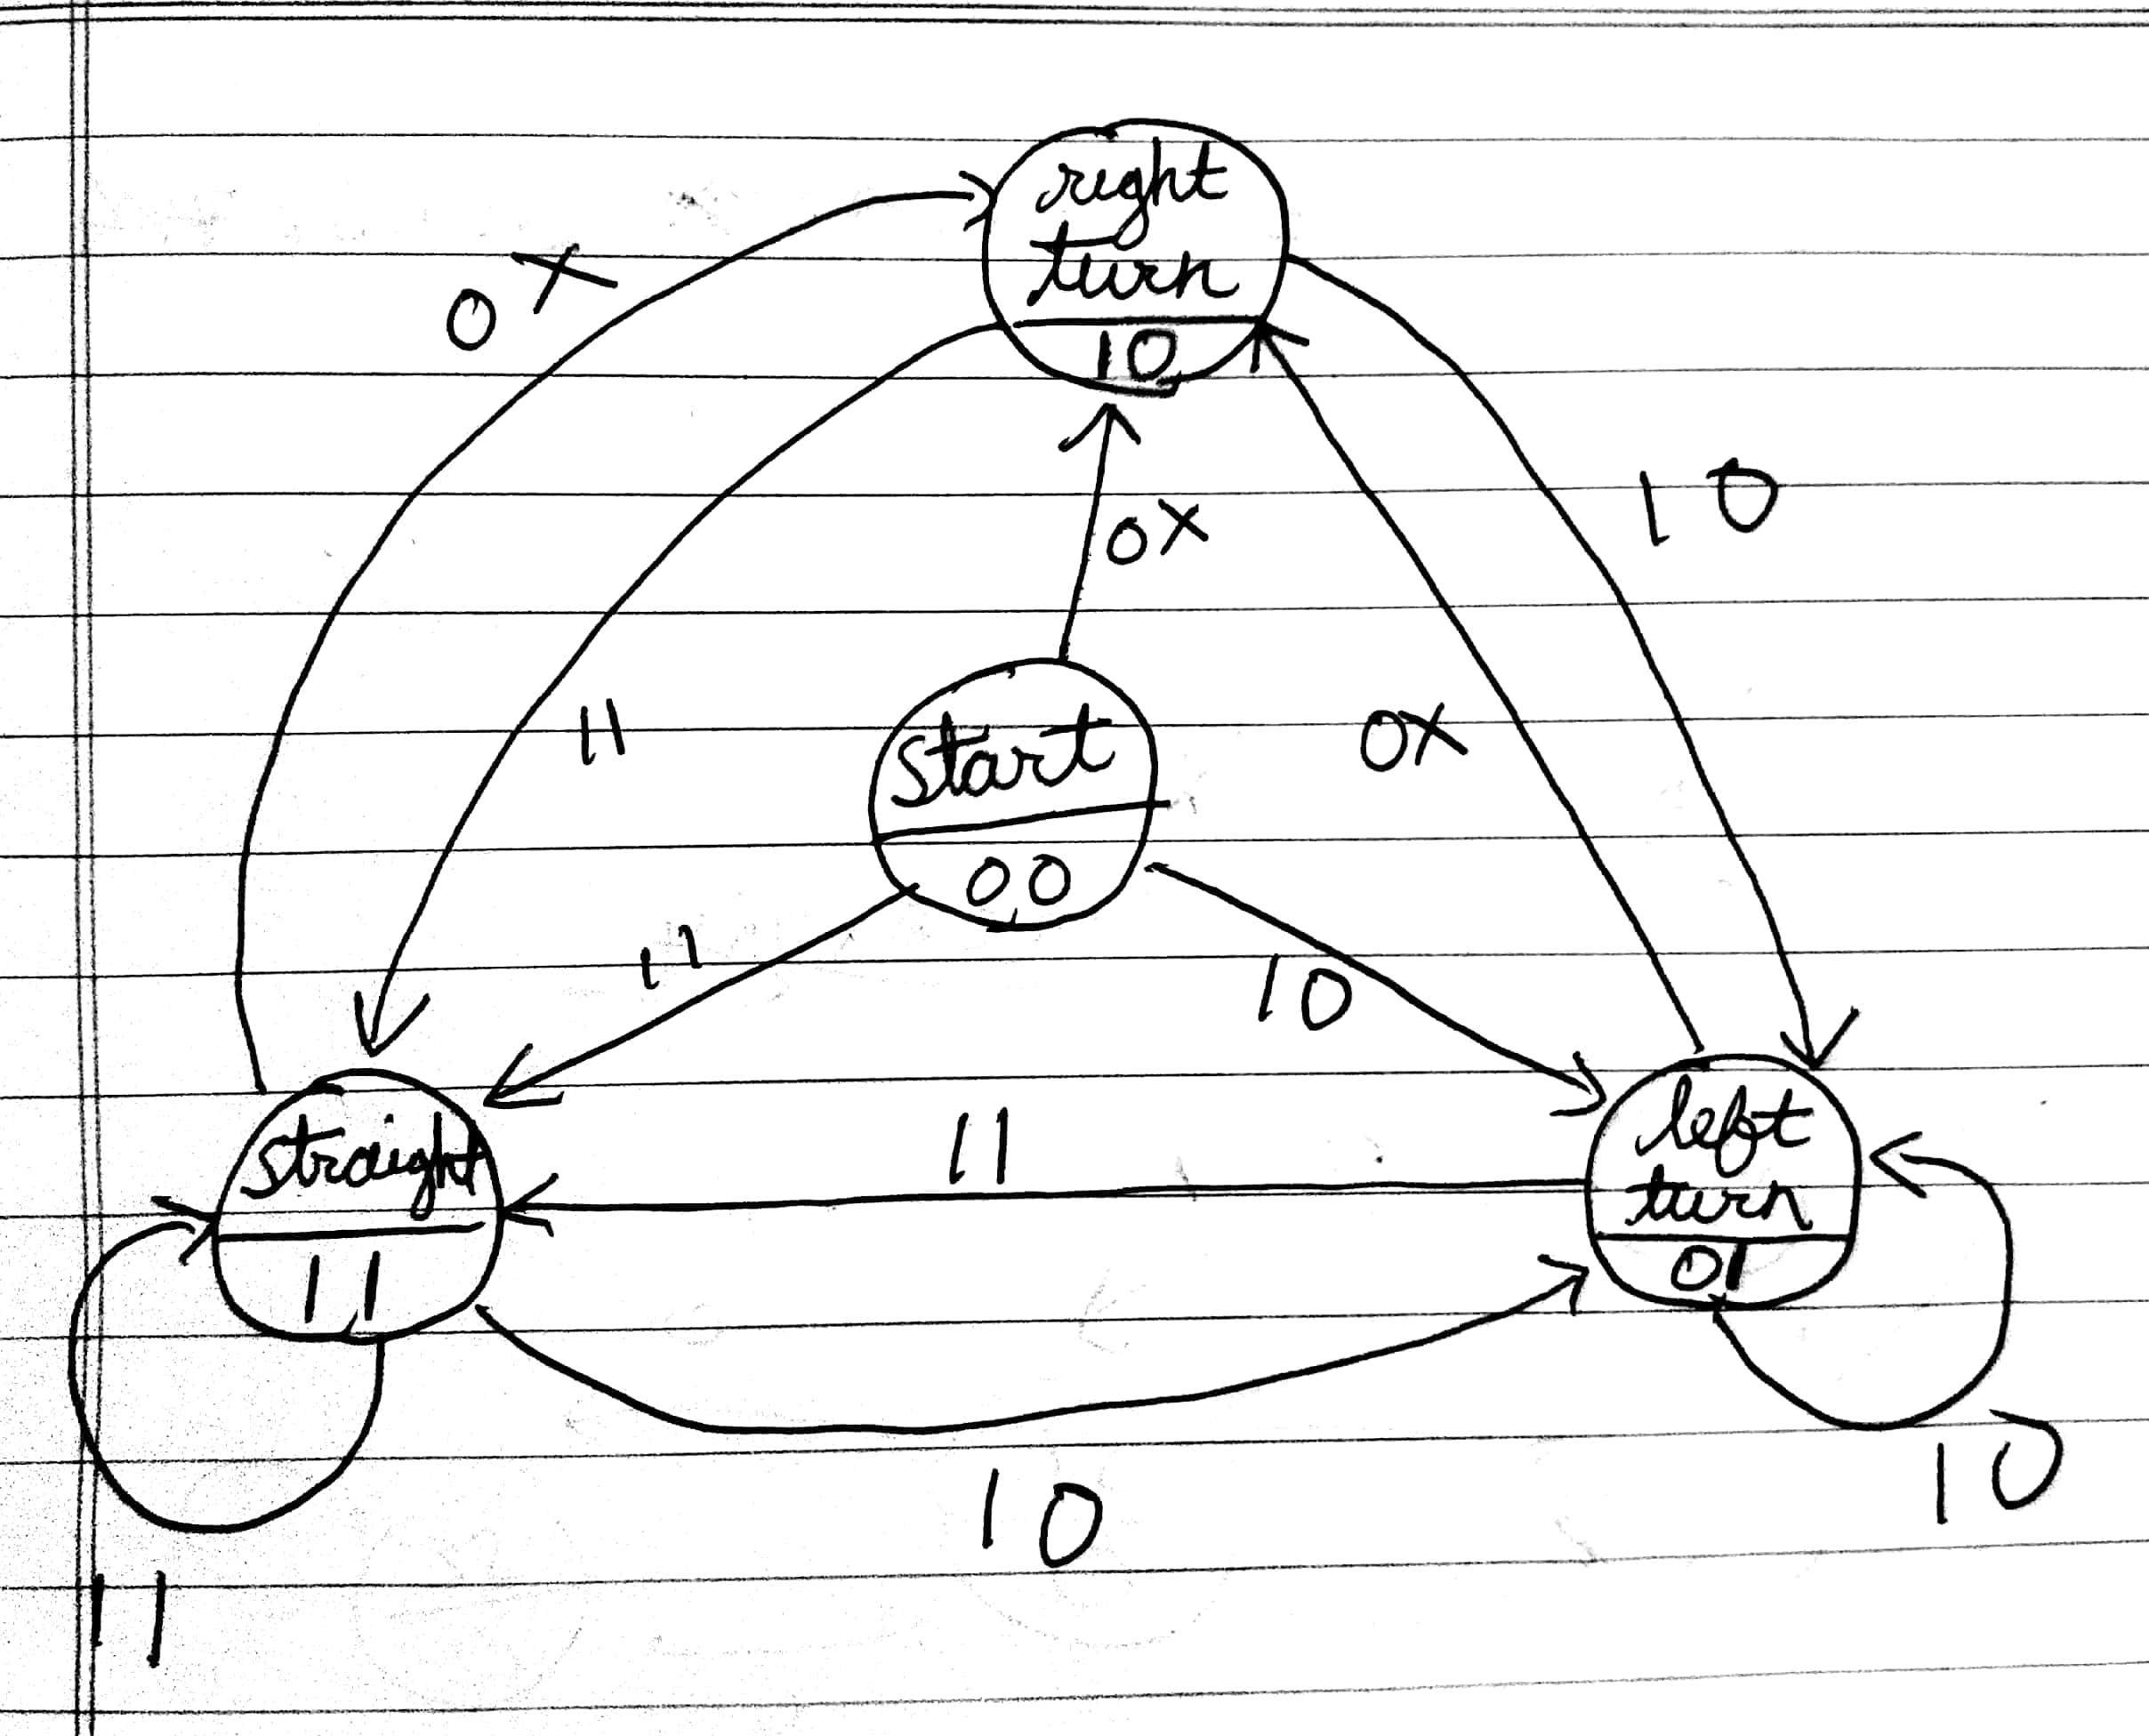
\includegraphics[scale=0.1]{images/q6fsm}
		\caption[]{FSM for Q6}
		\label{fig:q6fsm}
	\end{figure}
	
	\begin{figure}[H]
		\centering
		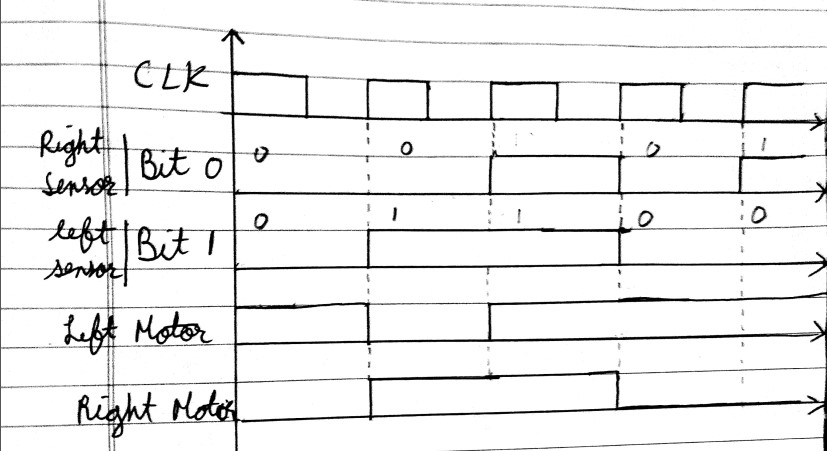
\includegraphics[width=1\linewidth]{images/q6timing}
		\caption[]{Timing Diagram for Q6}
		\label{fig:q6timing}
	\end{figure}
	\section*{Question 7}
	Consider a FSM that will receive input from a keypad and lock/unlock a door:\\
	1. The keypad has digits 0...9. \\
	2. On power up, the door is locked. \\
	3. As soon as the sequence 1, 1, 3, 8 is entered, the door must be unlocked.\\
	4. Once in a not locked state, when 0 is entered, the door is immediately locked and the FSM returns to a state in which it is waiting for a code.\\
	5. As soon as the sequence 1, 1, 3, 0 is entered, the FSM sounds an alarm and the door is permanently locked.\\
	6. Sequences other than the two listed above are ignored.\\
	7. The events are: 0, 1, ...9.\\
	8. The actions are: LOCK, UNLOCK, ALARM and none (X).\\
	Draw the diagram that describes the behaviour of this FSM.\\
	\begin{figure}[H]
		\centering
		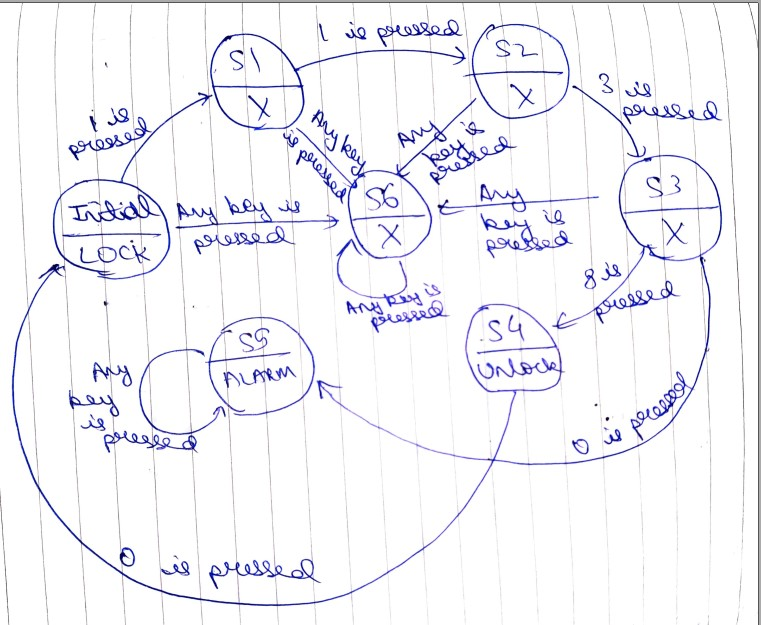
\includegraphics[scale=0.7]{images/q7fsm}
		\caption[]{FSM for Q7}
		\label{fig:q7fsm}
	\end{figure}
	\begin{figure}[H]
		\centering
		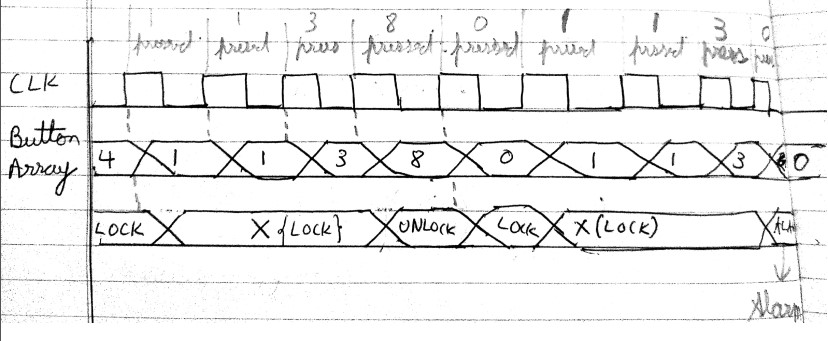
\includegraphics[width=1\linewidth]{images/q7timing}
		\caption[]{Timing Diagram for Q7}
		\label{fig:q7timing}
	\end{figure}
\end{document}